\section{Results}
\label{sec:results}
\begin{table*}[t]
\centering
\caption{Robustness summary by model and prompt condition. Higher \texttt{UNS\_hit Mean} is better; lower overlap and parse error are better. Best \texttt{UNS\_hit Mean} per model is in \textbf{bold}.}
\label{tab:robust_summary}
\resizebox{\textwidth}{!}{%
\begin{tabular}{@{}llrrrrrr@{}}
\toprule
Model & Condition & $N$ & \texttt{UNS\_hit Mean} & Overlap Hit Rate & Reddit Hits Mean & Match Rate & Parse Error Rate \\
\midrule
\gptfourone & Baseline & 18 & 0.562 & 0.389 & 24.667 & \textbf{0.889} & \textbf{0.000} \\
\gptfourone & Anti-Consensus & 18 & 0.542 & 0.222 & 6.722 & 0.778 & \textbf{0.000} \\
\gptfourone & Anti-Consensus+Reasoned & 18 & \textbf{0.669} & 0.111 & 8.167 & 0.722 & \textbf{0.000} \\
\midrule
\gptfive & Baseline & 18 & \textbf{0.468} & 0.333 & 11.278 & \textbf{0.667} & 0.167 \\
\gptfive & Anti-Consensus & 18 & 0.421 & \textbf{0.000} & \textbf{0.000} & 0.056 & 1.000 \\
\gptfive & Anti-Consensus+Reasoned & 18 & 0.400 & \textbf{0.000} & \textbf{0.000} & 0.000 & 1.000 \\
\bottomrule
\end{tabular}%
}
\end{table*}

\begin{table}[t]
\centering
\caption{Paired robustness tests (\texttt{UNS\_hit}). No comparison remains significant after Holm correction.}
\label{tab:robust_tests}
\resizebox{\linewidth}{!}{%
\begin{tabular}{@{}llrrrr@{}}
\toprule
Model & Comparison & $\Delta$\texttt{UNS\_hit} & Permutation $p$ & Holm-adjusted $p$ & Cohen's $d$ \\
\midrule
\gptfourone & Baseline vs Anti-Consensus & -0.020 & 0.826 & 0.826 & -0.052 \\
\gptfourone & Baseline vs Anti-Consensus+Reasoned & +0.107 & 0.141 & 0.492 & +0.358 \\
\gptfive & Baseline vs Anti-Consensus & -0.047 & 0.347 & 0.694 & -0.228 \\
\gptfive & Baseline vs Anti-Consensus+Reasoned & -0.068 & 0.123 & 0.492 & -0.387 \\
\bottomrule
\end{tabular}%
}
\end{table}


\begin{figure*}[t]
    \centering
    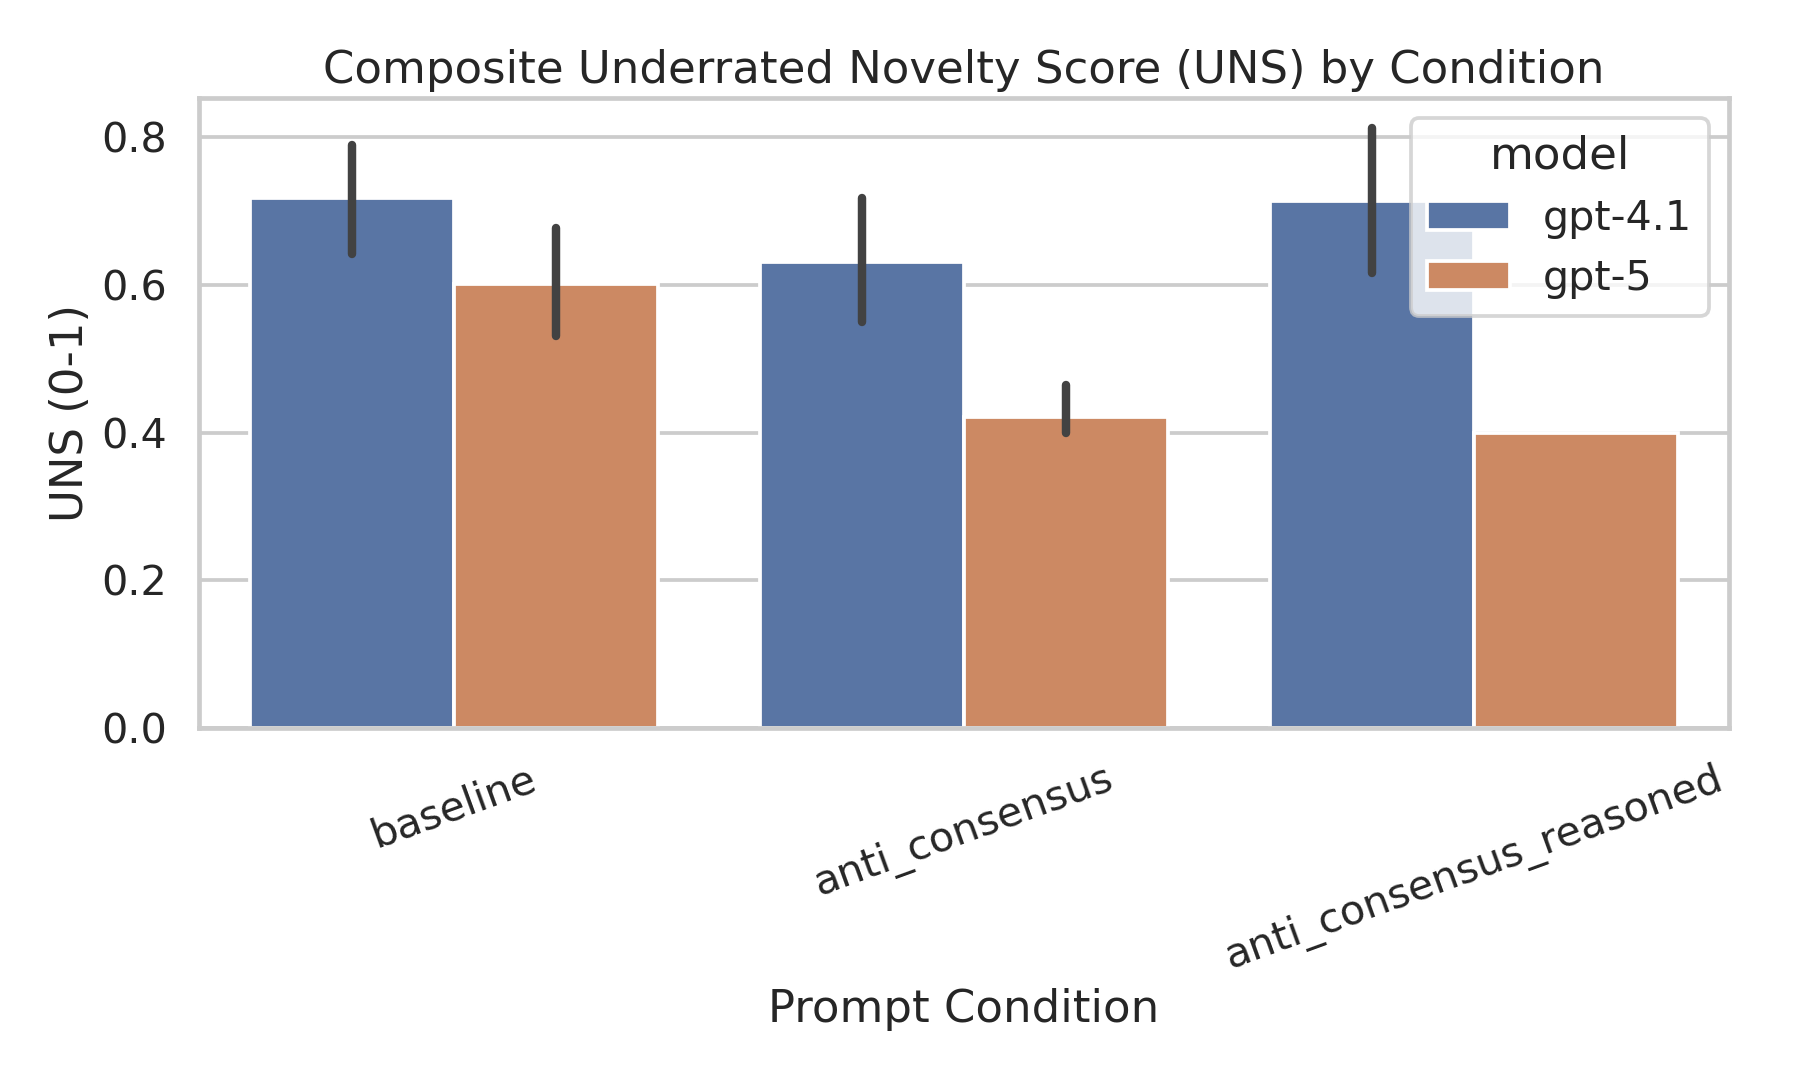
\includegraphics[width=0.32\textwidth]{figures/uns_by_condition_model.png}\hfill
    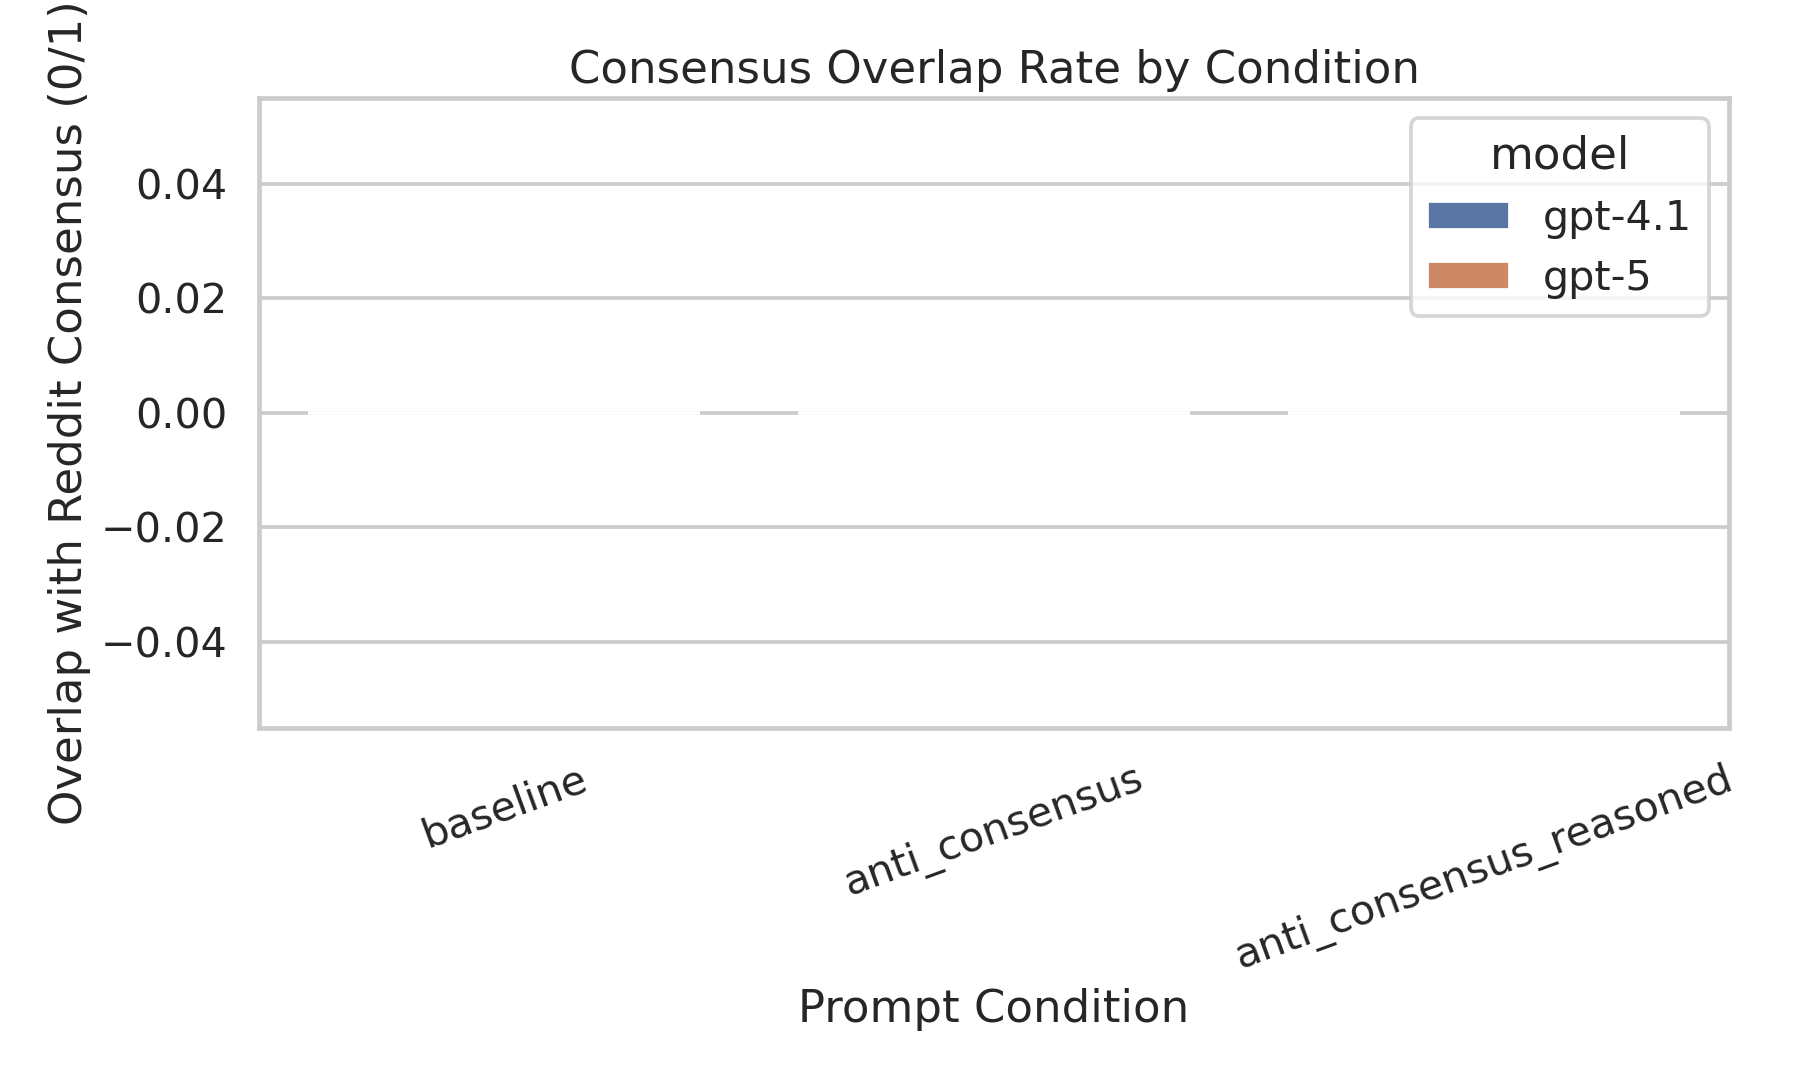
\includegraphics[width=0.32\textwidth]{figures/consensus_overlap_by_condition_model.png}\hfill
    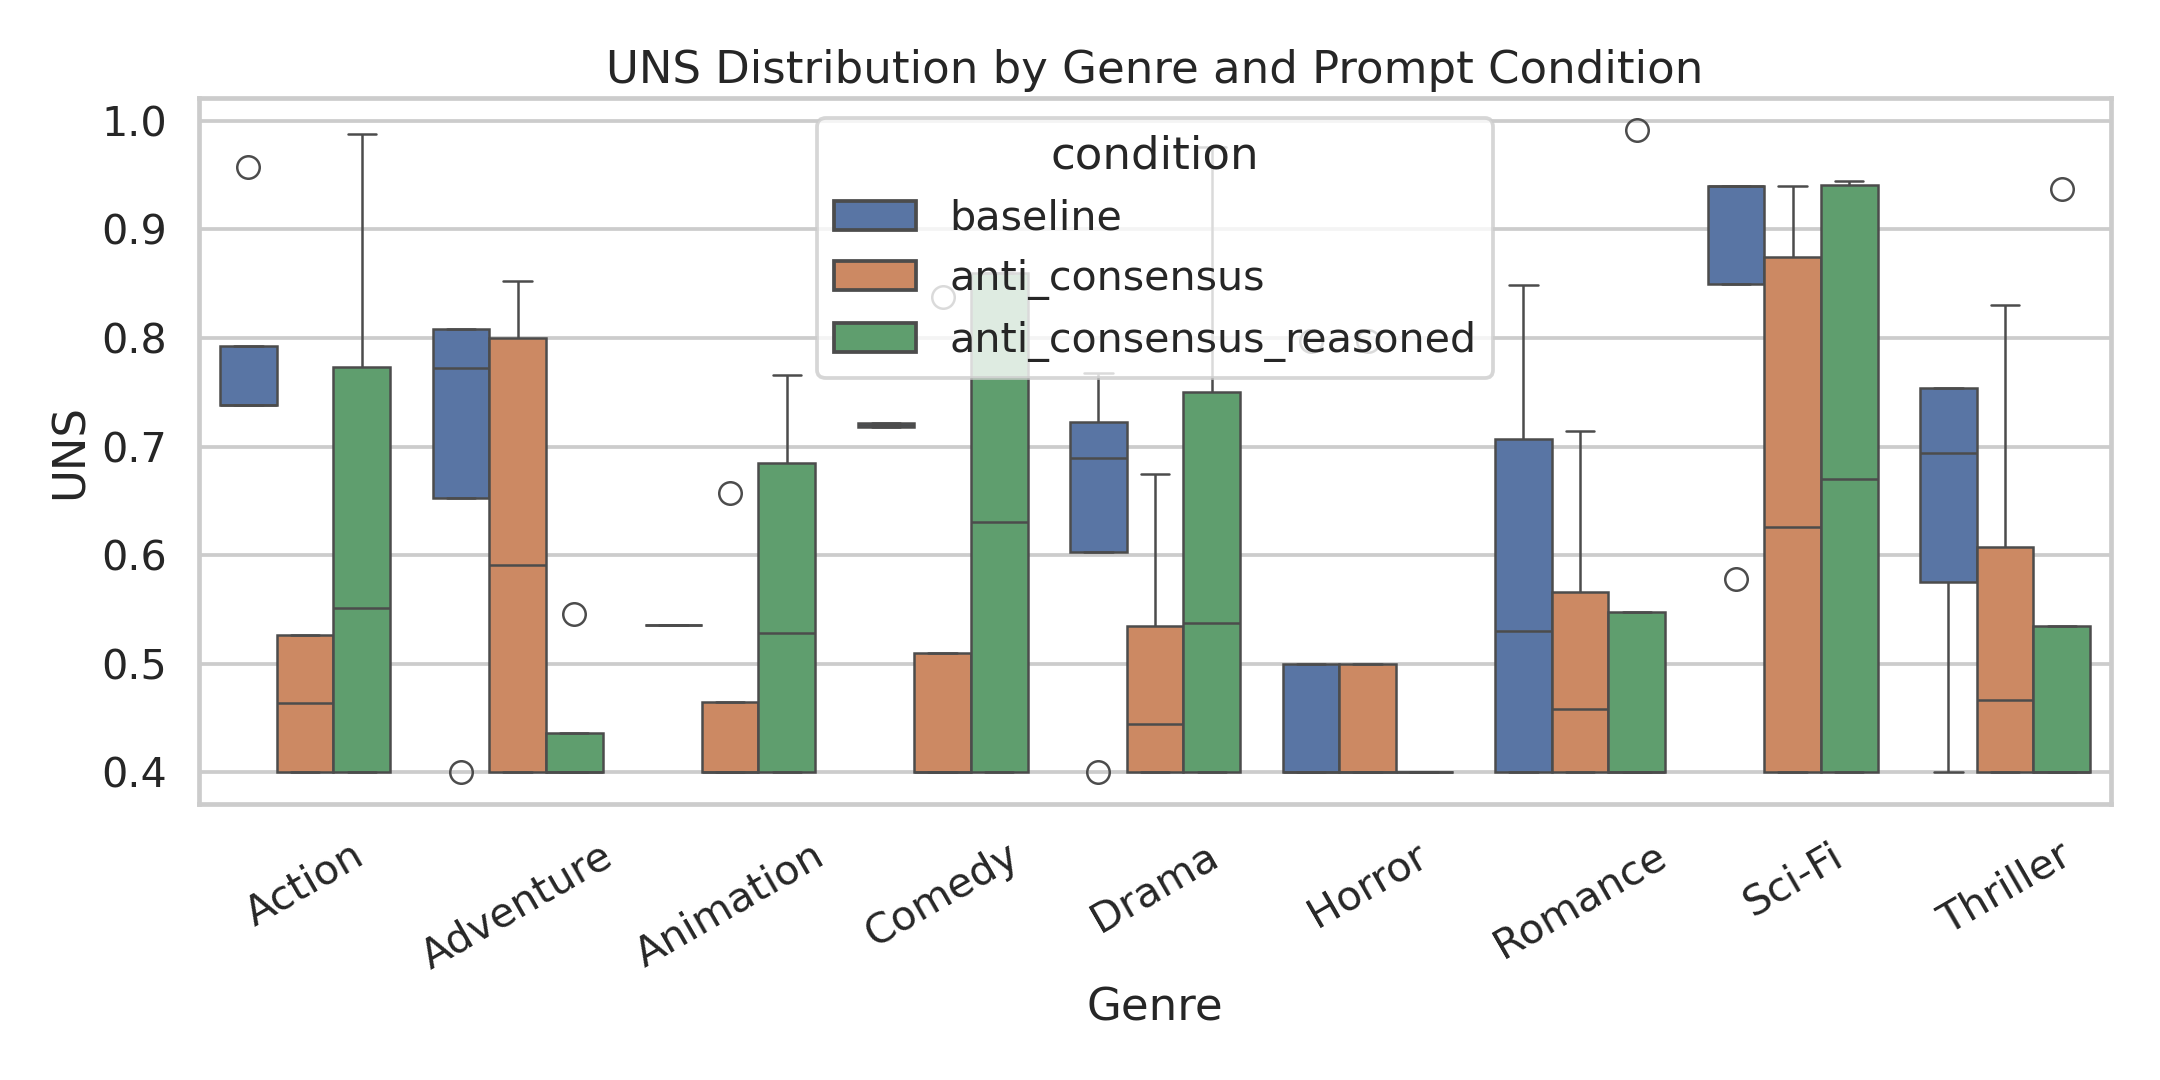
\includegraphics[width=0.32\textwidth]{figures/uns_by_genre_condition_boxplot.png}
    \caption{Robustness visualizations. Left: \texttt{UNS\_hit} by model and condition. Middle: overlap behavior by condition. Right: genre-level variability of \texttt{UNS\_hit}. Together, the plots show directional overlap reduction for \gptfourone under anti-consensus prompting, alongside substantial variance and non-significant corrected tests.}
    \label{fig:robust_plots}
\end{figure*}

\para{Main quantitative findings.} \Tabref{tab:robust_summary} shows clear directional changes for \gptfourone. Moving from baseline to anti-consensus+reasoned reduces overlap-hit rate from 0.389 to 0.111 and increases mean \texttt{UNS\_hit} from 0.562 to 0.669 (+0.107). Baseline to anti-consensus also reduces overlap (0.389 to 0.222), but with a slight mean \texttt{UNS\_hit} decrease (-0.020).

\para{Statistical tests.} \Tabref{tab:robust_tests} reports paired permutation tests with Holm correction. The largest positive effect is \gptfourone baseline vs anti-consensus+reasoned (Cohen's $d=+0.358$), but adjusted $p=0.492$, so it is not statistically significant at $\alpha=0.05$. No comparison survives correction.

\para{Model-specific robustness differences.} \gptfive baseline produces usable outputs (match rate 0.667, parse error 0.167), while both anti-consensus variants collapse in structured extraction (parse error 1.000). This failure mode dominates downstream metrics and explains why \gptfive overlap-hit rates appear low yet \texttt{UNS\_hit} does not improve.

\para{Ablation-style interpretation across prompt conditions.} Treating prompt condition as an intervention ablation, anti-consensus instructions reduce social obviousness for \gptfourone but do not guarantee higher composite novelty. Adding reasoned justification improves \texttt{UNS\_hit} directionally and yields the best overlap reduction for \gptfourone, suggesting that anti-consensus guidance plus rationale constraints is the strongest of the tested prompt variants.
